\begin{figure}[H]	
  \centering
    \resizebox{\linewidth}{!}{\tikzset{font=\Huge}\documentclass{standalone}
\usepackage{tikz}
\usepackage{aeguill}
\begin{document}
% generated by Plantuml 1.2018.12      
\definecolor{plantucolor0000}{RGB}{254,254,206}
\definecolor{plantucolor0001}{RGB}{168,0,54}
\definecolor{plantucolor0002}{RGB}{173,209,178}
\definecolor{plantucolor0003}{RGB}{0,0,0}
\definecolor{plantucolor0004}{RGB}{169,220,223}
\begin{tikzpicture}[yscale=-1
,pstyle0/.style={color=plantucolor0001,fill=plantucolor0000,line width=1.5pt}
,pstyle1/.style={color=plantucolor0001,fill=plantucolor0002,line width=1.0pt}
,pstyle2/.style={color=plantucolor0001,line width=1.5pt}
,pstyle4/.style={color=plantucolor0001,line width=1.0pt}
]
\draw[pstyle0] (6pt,14.5pt) rectangle (81.7514pt,62.5pt);
\draw[pstyle1] (21pt,30.5pt) ellipse (11pt and 11pt);
\node at (21pt,30.5pt)[]{\textbf{\Large C}};
\node at (35pt,23.5156pt)[below right,color=black]{Client};
\draw[pstyle2] (7pt,46.5pt) -- (80.7514pt,46.5pt);
\draw[pstyle2] (7pt,54.5pt) -- (80.7514pt,54.5pt);
\draw[pstyle0] (167pt,8pt) rectangle (267pt,68.8047pt);
\draw[color=plantucolor0001,fill=plantucolor0004,line width=1.0pt] (182pt,24pt) ellipse (11pt and 11pt);
\node at (182pt,24pt)[]{\textbf{\Large A}};
\node at (196pt,17.0156pt)[below right,color=black]{\textit{Prototype}};
\draw[pstyle2] (168pt,40pt) -- (266pt,40pt);
\draw[pstyle2] (168pt,48pt) -- (266pt,48pt);
\node at (173pt,52pt)[below right,color=black]{\textit{createClone()}};
\draw[pstyle0] (25pt,130pt) rectangle (199.2194pt,190.8047pt);
\draw[pstyle1] (40pt,146pt) ellipse (11pt and 11pt);
\node at (40pt,146pt)[]{\textbf{\Large C}};
\node at (54pt,139.0156pt)[below right,color=black]{ConcretePrototype1};
\draw[pstyle2] (26pt,162pt) -- (198.2194pt,162pt);
\draw[pstyle2] (26pt,170pt) -- (198.2194pt,170pt);
\node at (31pt,174pt)[below right,color=black]{createClone()};
\draw[pstyle0] (234pt,130pt) rectangle (408.2194pt,190.8047pt);
\draw[pstyle1] (249pt,146pt) ellipse (11pt and 11pt);
\node at (249pt,146pt)[]{\textbf{\Large C}};
\node at (263pt,139.0156pt)[below right,color=black]{ConcretePrototype2};
\draw[pstyle2] (235pt,162pt) -- (407.2194pt,162pt);
\draw[pstyle2] (235pt,170pt) -- (407.2194pt,170pt);
\node at (240pt,174pt)[below right,color=black]{createClone()};
\draw[pstyle4] (82.3943pt,38.5pt) ..controls (105.7252pt,38.5pt) and (135.9024pt,38.5pt) .. (161.7689pt,38.5pt);
\draw[color=plantucolor0001,fill=plantucolor0001,line width=1.0pt] (166.8814pt,38.5pt) -- (157.8814pt,34.5pt) -- (161.8814pt,38.5pt) -- (157.8814pt,42.5pt) -- (166.8814pt,38.5pt) -- cycle;
\node at (100.5pt,19.5pt)[below right,color=black]{Uses};
\draw[color=black,fill=black,line width=1.0pt] (138.8333pt,25.5664pt) -- (144.8333pt,28.5664pt) -- (138.8333pt,31.5664pt) -- (138.8333pt,25.5664pt) -- cycle;
\draw[pstyle4] (177.0769pt,84.8868pt) ..controls (164.1654pt,99.8888pt) and (150.1755pt,116.1437pt) .. (138.4875pt,129.7241pt);
\draw[pstyle4] (172.1519pt,79.8783pt) -- (190.5041pt,69.2858pt) -- (182.7631pt,89.0108pt) -- (172.1519pt,79.8783pt) -- cycle;
\draw[pstyle4] (256.5429pt,84.8868pt) ..controls (269.3314pt,99.8888pt) and (283.188pt,116.1437pt) .. (294.7648pt,129.7241pt);
\draw[pstyle4] (250.8912pt,89.0472pt) -- (243.2436pt,69.2858pt) -- (261.5454pt,79.9649pt) -- (250.8912pt,89.0472pt) -- cycle;
\end{tikzpicture}
\end{document}
}
\end{figure}
\subsection{Comparing Objects}
\begin{defnbox}\nospacing
  \begin{defn}[\javainline{obj1==obj2}]
    Compares references/addresses of the two operands.\\
  \end{defn}
\end{defnbox}
\begin{defnbox}\nospacing
  \begin{defn}[\javainline{obj1.equals(obj2)}]
    Compares the content of two objects.
  \end{defn}
\end{defnbox}
\begin{defnbox}\nospacing
  \begin{defn}[\javainline{obj1.getClass()==obj2.getClass()}]\label{defn:}
    Checks if two objects are of the same \rd{dynamic} type.
  \end{defn}
\end{defnbox}
\begin{defnbox}\nospacing
  \begin{defn}[\javainline{obj is instanceof}]
    Checks if an object is an instance of a class or interface.
  \end{defn}
\end{defnbox}
\begin{intentbox}[Intent of cloning]
  Provide a clone that satisfies:
  \begin{itemizenosep}
      \item New instance: \javainline{x.clone()!=x}
      \item Same dynamic type: \javainline{x.clone().getClass()==x.getClass()}
      \item Equal: \javainline{x.clone().equals(x)}
  \end{itemizenosep}
\end{intentbox}
\subsection{Deep vs. Shallow Copies}
\begin{figure}[H]
  \centering
  \vspace{-1em}
  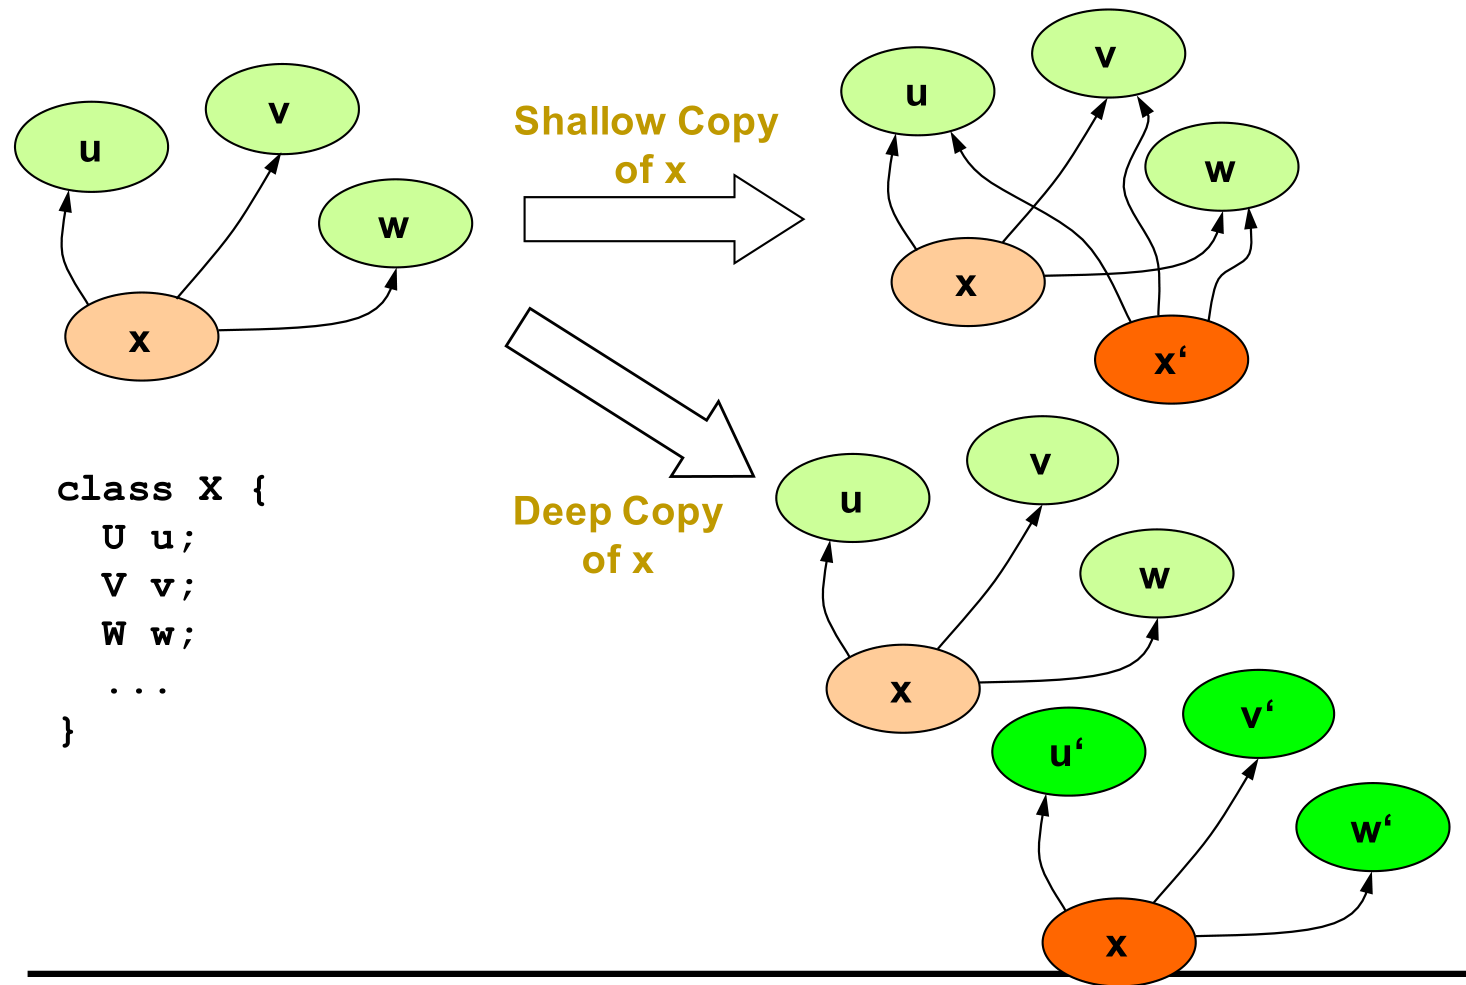
\includegraphics[width=1.0\columnwidth]{figures/shallowVsDeppCopy.png}
\end{figure}
\begin{defnbox}\nospacing
  \begin{defn}[Shallow Copy]\label{defn:shallowCopy}
    Is a bit-wise copy of an object. A new object is created that has an exact
    copy of the values in the original object.\\
    \imp{Thus}: If any of the fields of the object are references to other
    mutable types/objects, just the reference addresses are copied i.e., only
    the memory address is copied.\\
    \begin{mintlinebox}{java}
      myFoo.childObj == sFoo.childObj // ture
      myFoo.childObj.equals(sFoo.childObj) // ture
    \end{mintlinebox}
    \imp{Hence} manipulating child mutable types/objects of the copy will also modify the child mutable types/objects
    of the original object $\Rightarrow$ not a real copy.
  \end{defn}
\end{defnbox}
\begin{notebox}[Attention]\nospacing
  Lists are complex types!
\end{notebox}
\begin{codeboxNl}[Shallow list copy]{java}
  public class Ex { 
    private int[] data; 
    // makes a shallow copy of values 
    public Ex(int[] values) { 
        data = values; 
    } 
} 
\end{codeboxNl}
\begin{defnbox}\nospacing
  \begin{defn}[Deep copy]\label{defn:deepcopy}
    Recursively copies objects, and hence is a real copy.
    \begin{mintlinebox}{java}
      myFoo.childObj == sFoo.childObj // false
      myFoo.childObj.equals(sFoo.childObj) // ture
    \end{mintlinebox}
  \end{defn}
\end{defnbox}
\begin{codeboxNl}{java}
class Foo {
  private Bar myBar;
  ...
  public Foo shallowCopy() {
    Foo newFoo = new Foo();
    newFoo.myBar = myBar;
    return newFoo;
  }

  public Foo deepCopy() {
    Foo newFoo = new Foo();
    newFoo.myBar = myBar.clone();
    return newFoo;
  }
}

Foo myFoo = new Foo();  
Foo sFoo = myFoo.shallowCopy();  
Foo dFoo = myFoo.deepCopy();  

myFoo.myBar == sFoo.myBar => true  
myFoo.myBar.equals(sFoo.myBar) => true  
myFoo.myBar == dFoo.myBar => **false**  
myFoo.myBar.equals(dFoo.myBar) => true  
\end{codeboxNl}
\subsubsection{Java.lang.Clonable}
\label{subsubsec:Java.lang.Clonable}
\begin{defnbox}\nospacing
  \begin{defn}[Clonable]\label{defn:}
    Is a marker interface \cref{defn:markerInerface}, that is special in that
    it is empty and does not even declare the clone method:
    \begin{mintlinebox}{java}
      public interface Cloneable {
        // Marker interface
      }
    \end{mintlinebox}
    It is simply there to indicate that a class is clonable.
  \end{defn}
\end{defnbox}
\begin{codeboxNl}[java.lang.Object]{java}
protected Object clone() throws CloneNotSupportedException {
  if (!(this instanceof Cloneable)) {
    throw new CloneNotSupportedException(
      "Doesn't implement Cloneable interface!");
  }
  return VMMemoryManager.clone(this);
}
\end{codeboxNl}
\begin{codeboxNl}[VMMemoryManager]{java}
  class VMMemoryManager {
    static native Object clone(Object object);
    |\ldots|
  }
\end{codeboxNl}
\begin{defnbox}\nospacing
  \begin{defn}[\javainline{nativ}]
    Enables java code running JVM to call\& be called by nativ applications
    (programs specific to hardware\&OS platform) and libraries written in other
    languages e.g.\ C.\\
    \imp{Here}: it calls C-code that uses \cppinline/memcpy/ to
    copy the given object \rd{bitwise} efficiently ($\Rightarrow$ \rd{shallow copy}).
  \end{defn}
\end{defnbox}
\subsubsection{Java.lang.Object and Clonable}
\begin{defnbox}\nospacing
  \begin{defn}[Java.lang.Object]\label{defn:}
    Is the base class of all Classes and provides a \javainline{protected}
    default implementation of the \javainline{clone} method which:
    \begin{itemizenosep}
      \item Throws an \javainline{CloneNotSupportedException}
      if an object of a class calls the clone method without
      implementing the \javainline{Cloneable} marker interface
      \item Will lead to a compile time error if we try to copy an object
      not from within itself, subclasses, or classes of the same package.\\
      This is because clone is \javainline{protected}
    \end{itemizenosep}
  \end{defn}
\end{defnbox}
\begin{defnbox}[How to use:]\nospacing
    \javainline{java.lang.Object.clone} the right way:
    \begin{itemizenosep}
        \item If the Class we want to clone only contains primitive fields or
      references to \javainline{immutable} objects, then we can simply:\\
      \rdb{Shallow Copy}:
      \begin{itemize}
          \item override the \javainline{clone} method as a public method
          \item call \javainline{super.clone()} to make a shallow copy using \cppinline/memcpy/
      \end{itemize}
      \begin{mintlinebox}{java}
        |\optc{visibility}| class MyClass implements Cloneable{
          |\optldots|
          public Object clone(){
            |\ul[ulc2]{try}|{
              // go up in hierarchy until
              // java.lang.Object.clone
              MyClass c = |\ul{(MyClass)}| super.clone();
              return c;
            } catch (CloneNotSupportedException e){
              throw new InternalError(e.getMessage());
            }
          }
        }
      \end{mintlinebox}
    \end{itemizenosep}
\end{defnbox}
\begin{notebox}[Notes]\nospacing
  \begin{itemizenosep}
      \item \ul{Type Conversion}: MyClass may be a subclass of another class
    i.e.\ the parent class will call again \javainline{super.clone} until
    we reach \javainline{java.lang.object}.\\
    Hence we need to make sure that we will obtain the right dynamic type
    (\javainline{x.clone().getClass()==x.getClass()}).
      \item \ul[ulc2]{try}: again if MyClass is a subclass of other, the
      super/parent classes need to implement at least the \javainline{clonable}
      marker interface (do not necessarily need to implement clone method).
  \end{itemizenosep}
\end{notebox}
\begin{defnbox}\nospacing
  \begin{itemizenosep}
    \item If the Class we want to clone does contains complex fields or
    references to \javainline{mutable} types then we need to:\\
      \rdb{Deeply Copy}:
    \begin{itemize}
        \item Recursively clone all elements
        \item Replace lists with new ones
    \end{itemize}
  \end{itemizenosep}
\end{defnbox}
\begin{codeboxNl}[Company: Deep Copy]{java}
public class Company implements Cloneable {
  private String name;
  // Java lists are mutable data types!
  private ArrayList<Employee> employees = new ArrayList<>();
  public Object clone() {
    try {
      Company c = (Company) super.clone();
      c.employees = new ArrayList<>();
      for(Employee e : employees)     
        c.employees.add(e.clone());
      return c;
    } catch (CloneNotSupportedException e) {
      throw new InternalError(e.getMessage());
    }
  }     
}
\end{codeboxNl}
\begin{codeboxNl}[Employee: Shallow Copy]{java}
public class Employee implements Cloneable {
  // Only primitive types
  private String name;
  private int yearOfBirth;
  public Object clone() {
    try {
      return super.clone();
    } catch (CloneNotSupportedException e) {
      throw new InternalError(e.getMessage());
    }
  }
}
\end{codeboxNl}
\begin{notebox}[Why is clone protected?]\nospacing
  \begin{itemizenosep}
      \item 
  Clone is declared protected so that if all we do is implement Cloneable, only
  subclasses and members of the same package will be able to invoke clone() on
  the object.\\
  To enable any class in any package to access the clone() method, you'll have
  to override it and declare it \javainline{public}! 
      \item Clone cannot be invoked on objects of static type Object.
  \end{itemizenosep}
\end{notebox}
\begin{codeboxNl}[Compile Time Error]{java}
  import myClass
  // Implementing (empty) marker interface
  // But does not implement clone method

  class Client{
    public static void main(String[] args){
      myClass obj1 = new myClass();
      // Compile time error => calling protected method
      myClass obj2 = obj1.clone();
      
    }
  }
\end{codeboxNl}
\begin{notebox}[Notes]\nospacing
  \begin{itemizenosep}
      \item Java allows covariant typing \label{defn:covariantTying}
      \item Alias references and cycles have to be handled manually
  \end{itemizenosep}
\end{notebox}
\subsubsection{Clone with copy Constructor}
\begin{sectionbox}\nospacing
  Java does not provide a default copy constructor as in C++ but we may write
  one and then use it for our clone method.
\end{sectionbox}
\begin{codeboxNl}[Clone with copy constructor]{java}
class Company {
  public Company(Company c) {
    if(c==null) throw new IllegalArgumentException();
      // initialize this with attributes of c
    }
    |\optldots|
    public Company clone() {
      return new Company(this);
    }
}
\end{codeboxNl}
\begin{notebox}[Notes]\nospacing
  \begin{itemizenosep}
      \item It is possible that the state of an immutable type
       changes after creation, as long as this change is not visible to the
       client.
      \item Companion mutables: provide conversion classes e.g.\
    immutable \javainline{string} and mutable \javainline{stringBuffer}
  \end{itemizenosep}
  Provide conversionhh
\end{notebox}
\subsubsection{Prototype Design Pattern}
\begin{figure}[H]
  \centering
  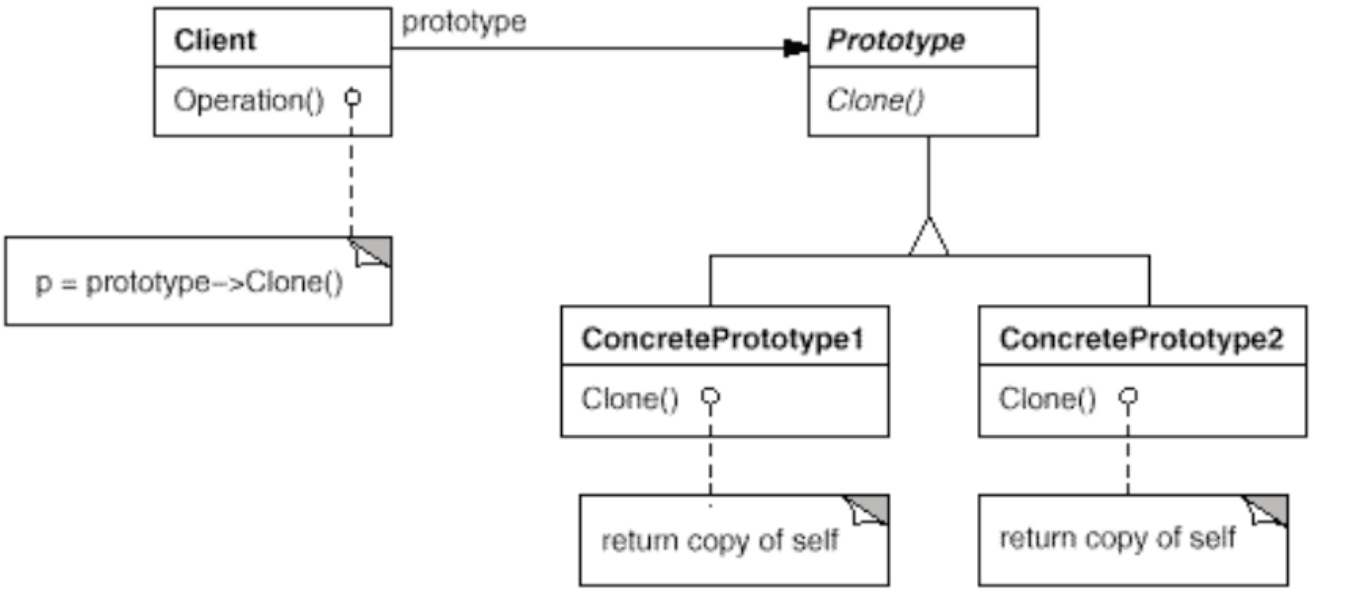
\includegraphics[width=1.0\columnwidth]{figures/prototypePattern.png}
\end{figure}
\begin{sectionbox}[Problem]\nospacing
  New object creation \javainline{MyClass obj = new MyClass()} is costly e.g.\
  an object is created by calling a costly database operation inside the constructor.\\
  Thus if we need many similar types it is not a good idea to always construct a
  new object using \javainline{new}.
\end{sectionbox}
\begin{intentbox}[Intent]
    Avoid costly creation of an object using \javainline{new} by \textit{cloning
      it from some similar prototype} and simply adapt it to our needs.\\
    \imp{Thus}: we specify the kinds of objects to create using a prototypical
    instance, and create new objects by cloning the right prototype.
\end{intentbox}
\begin{partbox}[Participants]
  \begin{itemizenosep}
      \item \imp{Prototype}:
      \item
      \begin{itemizenosep}
        \item Is in its easiest form the \javainline{java.lang.Clonable}
      interface
        \item An interface that implements the clonable interface
        \begin{itemize}
            \item Implements the clonable marker interface
            \item declares a public clone method
            \item may declare methods for other classes
        \end{itemize}
          \item An abstract class e.g.\ Shape implementing the
        \javainline{java.lang.Clonable} interface
      \end{itemizenosep}
        \item \imp{Concrete Prototype}: is an concrete class implementing the
      prototype interface that we may want to clone
        \item \imp{Client}: Produces new instances by calling clone on concrete
      prototypical prototypes.
  \end{itemizenosep}
\end{partbox}
\begin{notebox}[Note: Why not just use clonable interface]\nospacing
  Many consider clonable as broken/bad design as it does not even declare clone
  thus checking anything with the clonable marker interface does not bring us
  anything e.g.\
  \begin{mintlinebox}{java}
       concretPrototype a = new A();
       if(a instanceof Cloneable)
       {
         // This check is worthless and
         // the method may fail
           A copied = a.clone(); 
       }
  \end{mintlinebox}
\end{notebox}
\begin{codeboxNl}[Abstract Prototype]{java}
abstract class Prototype implements Cloneable {

  public Prototype clone() throws CloneNotSupportedException {
    return (Prototype) super.clone();
  }
  public abstract void setX(final shot X);
  public abstract short getX();
}
\end{codeboxNl}
\begin{codeboxNl}[Concrete Prototype]{java}
class ConcretePrototype implements Prototype {
  private int x;

  public ConcretePrototype extends Prototype {
    return (Prototype) super.clone();
  }

  public abstract void setX(int X){
    x = X;
  }

  public abstract short getX(){
    return x;
  }
}
\end{codeboxNl}
\begin{codeboxNl}[Client]{java}
public class Client{
  public static void main(String[] args) {
  Prototype origin =  new ConcretePrototype(10);
  Prototype clone =  origin.clone();
  clone.setX(4);
}
\end{codeboxNl}
\subsubsection{Exmple}
\label{subsubsec:Exmple}
\begin{codeboxNl}[Abstract Prototype]{java}
public abstract class Figure implements Cloneable {
  |\optldots|
  public Object clone() {
      Object clone = null;
      try {
         clone = super.clone();
      } catch (CloneNotSupportedException e) {
         e.printStackTrace();
      }
      return clone;
      // Or do not let clone abstract base class
    }
}
\end{codeboxNl}
\begin{codeboxNl}[Concrete Prototype]{java}
public class Rectangle extends Figure {
  |\optldots|
  public Object clone() {
      Object clone = null;
      try {
         clone = super.clone();
         // or provide deep copy
      } catch (CloneNotSupportedException e) {
         e.printStackTrace();
      }
      return clone;
    }
}
\end{codeboxNl}
\begin{codeboxNl}[Client]{java}
public class Client{
  |\optldots|
  Rectangle greenRec = new Rectangle(green);
  Circle blueCircle = new Circle(blue);
  Circle yellowCircle = new Circle(yellow);

  public static void main(String[] args) {
    Rectangle myRecClone = greenRec.clone();
    Circle myCircleClone = yellowCircle.clone();
  }
\end{codeboxNl}
%%% Local Variables:
%%% mode: latex
%%% TeX-master: "../formulary"
%%% End:
